\section{Introduction}
\label{sec:Introduction}

\subsection{Motivation}

The larger goal of our work is to support efficient information access on complex topics. 
%
For example, consider a journalist writing an article on the recent Coronavirus Disease 2019 (COVID-19)
pandemic in which she analyzes the different angles of the pandemic on the economy and worker's safety. COVID-19 has been widely discussed in the news, social media, and research commentary in various aspects such as transmission, pathology, experimental treatment, food safety, protests, and stay-at-home-orders. So the journalist has to sift through hundreds of associated texts to identify those that discuss the right context. The journalist finds it challenging to identify different texts that are relevant for her article without being overwhelmed with other aspects of COVID-19. Of course, keyword searches help her, but she would also like to understand the larger connections between her topic and other policies, research findings, and incidents. One relevant text passage for her task is displayed in Figure \ref{fig:introexample}, top. 



\begin{figure}
\justify
\begin{quote}
Several \textbf{meat processing plants} around the \textbf{U.S.} are sitting idle this week because workers have been infected with the \textbf{coronavirus}. \textbf{Tyson Foods}, one of the country's biggest \textbf{meat processors}, says it suspended \textbf{operations} at its \textbf{pork plant} in \textbf{Columbus Junction, Iowa}, after more than two dozen workers got sick with \textbf{COVID-19}. \textbf{National Beef Packing} stopped \textbf{slaughtering} \textbf{cattle} at another \textbf{Iowa} plant, and \textbf{JBS USA} shut down work at a \textbf{beef plant} in \textbf{Pennsylvania}.
\end{quote}

\begin{small}
\begin{itemize}
\item Meat packing industry:  Meatpackers / Today
\item United States: Culture / Food
\item Coronavirus Disease 2019: Cause / Transmission
\item Tyson Foods: Controversies / Coronavirus (COVID-19) pandemic
\item Continuous production: Shut-downs / Safety
\item Columbus Junction, Iowa: History
\item National Beef: Food Safety
\item Cattle: Economy / Cattle meat production
\item Iowa: Economy / Manufacturing
\item Meat Industry: Effects on Livestock Workers
\item Animal Slaughter: National laws / United States
\item JBS USA: Coronavirus Outbreak
\item Pennsylvania: Economy / Agriculture
\end{itemize}
\end{small}


\caption{Entity Aspect Linking Example. Top: An example paragraph about a COVID-19 outbreak in the meat packing industry, where the entity [Coronavirus Disease 2019] is mentioned with its aspect ``transmission''.  Bottom: Entities mentioned in text with their referenced aspects (here taken from Wikipedia sections). From the fine-grained entity aspect links, the relevance of this paragraph for the journalist's task emerges. The paragraph is taken from NPR \url{https://n.pr/35XMdli}.}
\label{fig:introexample}

\end{figure}


For such support systems, entity linking tools \cite{ferragina2010tagme,mendes2011dbpedia,piccinno2014wat} identify and disambiguate entity mentions, such as of the entity ``Coronavirus Disease 2019.'' However, the resulting entity links do not differentiate between different aspects of the entity that are being discussed. The journalist in the motivating example would be best helped with a fine-grained extension of entity links---we call this task entity aspect linking. Given a catalog of aspects for each entity, entity aspect linking predicts for each entity, which of its aspects is referenced in the context. 

 Figure \ref{fig:introexample} lists the most relevant entity aspects for the entities mentioned in the text above.  In this example, the catalog of entity aspects is derived from sections in the Wikipedia article of the mentioned entity---other sources for aspect catalogs can be a reputation management platform or journalistic notes, as long as a brief description of each aspect is available. We refer to this description as \emph{aspect content}.  
 
 For very popular topics such as COVID-19, aspect prediction can be addressed with lexicalized text classification. However, our goal is to develop a support system that also works for less popular topics, where the manual annotation of training data would defeat the purpose. 

Finally, the benefits of an entity-aspect-linker go much beyond classifying into different aspects of a single target entity (such as COVID-19). While knowledge graphs have shown a lot of advantages, entity aspect linking allows to build a sub-entity knowledge graph, where nodes represent entity aspects, which are grouped into entities. Because the aspects are associated with content that mentions other entities, we can establish relations between entity-aspects by entity-aspect-linking the content of aspects.


%\ld{Shubham delete when ok. Deleted Paragraph. I am not a fan of jobs and apple. If you later need an example to explain entity linking you can move it there -- in the introduction I would focus on stuff that's not very well known.}
% Entity Linking is the task of automatically annotating mentions of entities in text and linking them to their knowledge base entries. Given a sentence such as \textit{Steve Jobs founded Apple}, entity linking tools first aim to identify the entities in the sentence (such as \textit{Steve Jobs} and \textit{Apple}), and then to disambiguate the entity mentions (does the mention \textit{Apple} refer to the fruit or the company?). Finally, they link the mention to its knowledge base entry. For example, the mention \textit{Apple} would be linked to the knowledge base entry for \textit{Apple\_(Company)} and not \textit{Apple\_(Fruit)}.

% Consider a journalist  writing a report on the recent COVID-19 pandemic who wants to analyse the different angles in which it has been mentioned on social media such as the tweet \textit{Several states are seeing outbreaks of \#COVID19 in meat and poultry processing facilities}. To them, identification and disambiguation of the entity \textit{COVID-19} in text may not be enough. They would also want to know the different roles the entity plays. For example, does the mention of COVID-19 in the tweet above refer to its \textit{transmission}, \textit{pathology}, or \textit{experimental treatment}? 

%\ld{Merged paragraphs below.}
% Current entity linking tools \cite{ferragina2010tagme,mendes2011dbpedia,piccinno2014wat} can correctly identify and disambiguate entities in text. However, they cannot infer the correct \textit{aspect} of the entity from the context. For example, given the sentence, \textit{Boris Johnson is back after recovering from COVID-19}, an entity linking tool can correctly disambiguate and link the mention \textit{Boris Johnson} to its knowledge base entry but cannot infer whether the mention refers to his role as a \textit{Writer at the Daily Telegraph} or as the \textit{Prime Minister of the UK}. In general, an entity mention may be related to several different events, roles, and topics. We refer to each of them as an \textit{Entity Aspect}. 

\noindent In this work we focus on improving entity aspect linking:

\paragraph{\textbf{Entity Aspect Linking Task.}} Given a mention $M_E$ for entity $E$ in a context $C$ such a tweet, sentence or paragraph and a set of $n$ predefined aspects $A_{E} = \{A_1, A_2, A_3, \cdots, A_n\}$ along with their contents, link the mention $M_E$ to an aspect $A_i \in A_{E}$ that best captures the addressed topic. 

\bigskip
%\ld{TODO! I keep on referring to context and content, I think we need a figure for that.}
In the following, we distinguish between context and content: the context is the text surrounding the entity mention we seek to aspect-link. With content, we refer to content associated with the aspect. This is depicted in Figure \ref{fig:context-vs-content}.

\begin{figure}
    \centering
    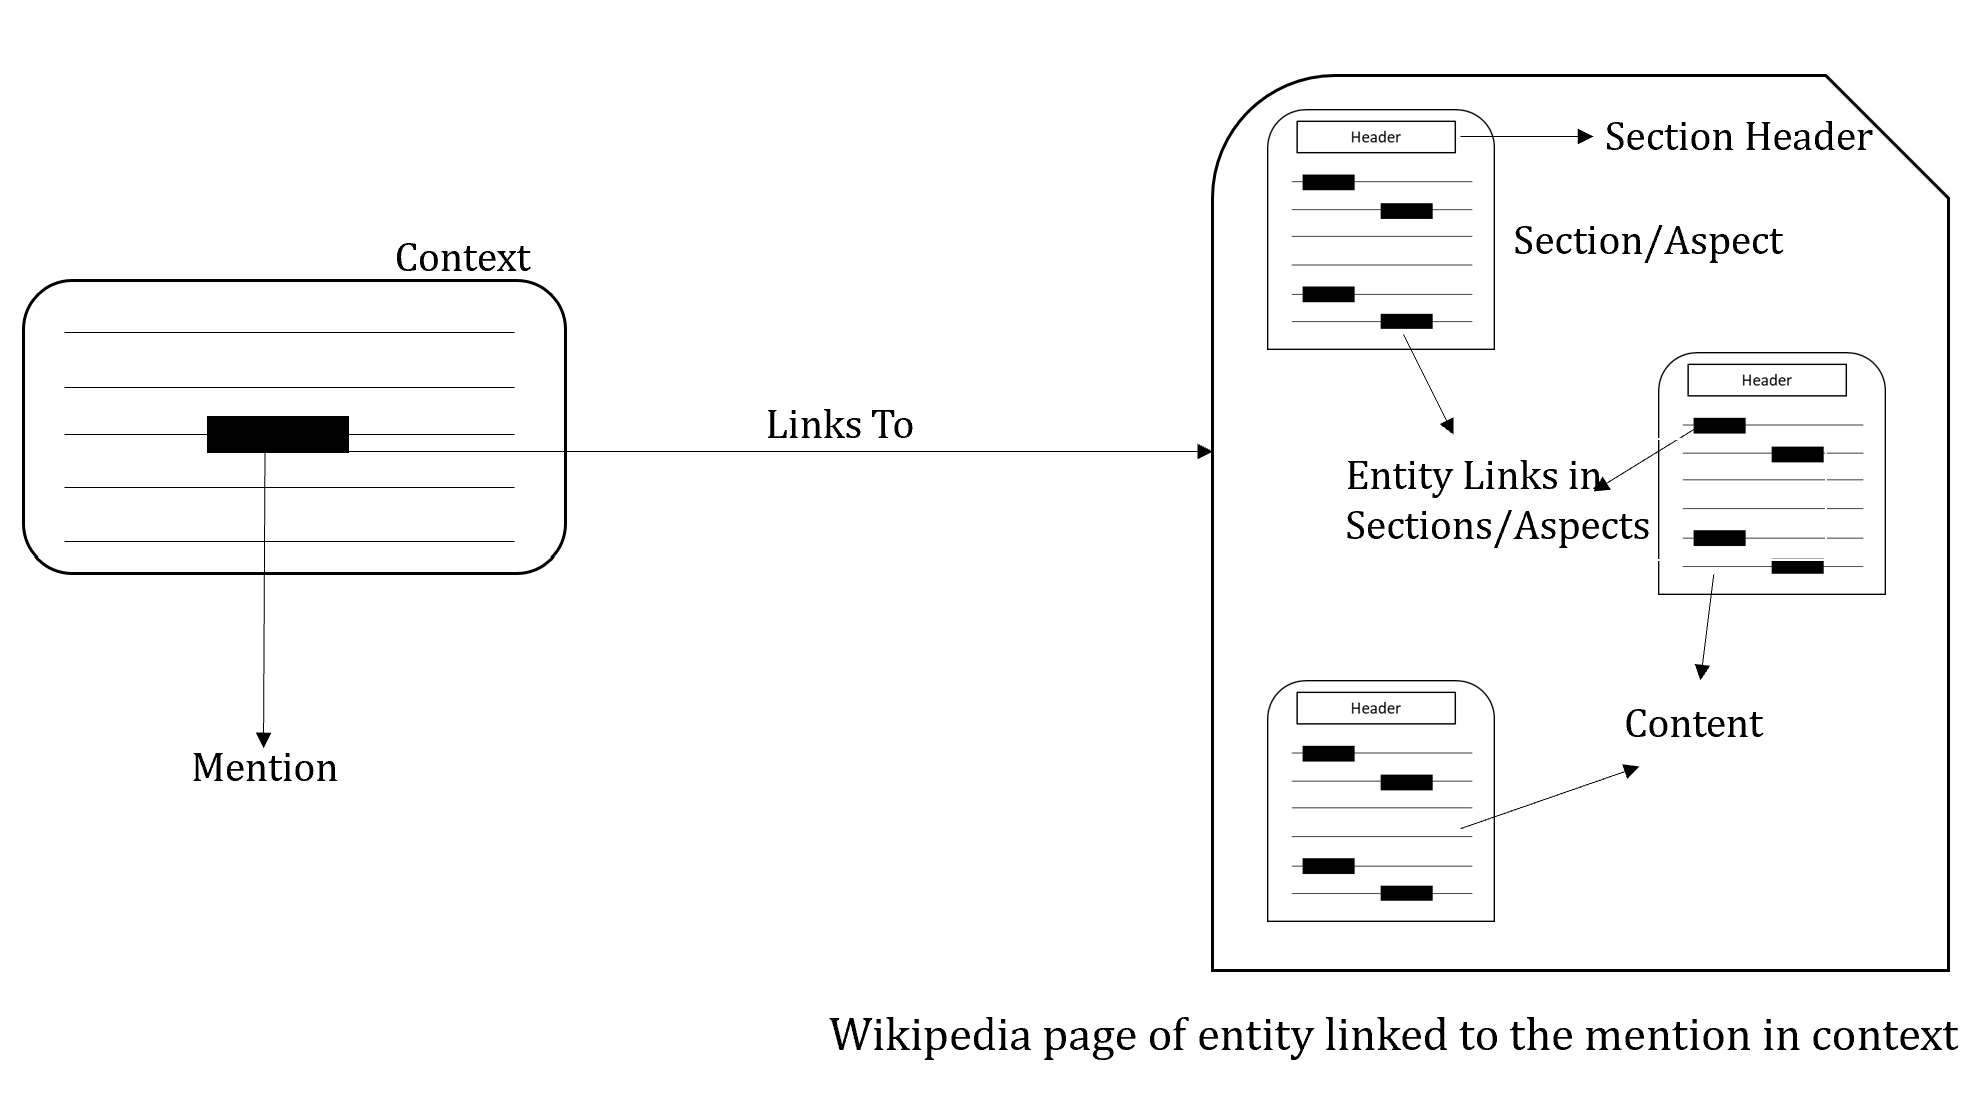
\includegraphics [scale=0.6]{context-and-content.png}
    \caption{Graphical representation of various concepts in aspect linking.}
    \label{fig:context-vs-content}
\end{figure}

Nanni et al. \cite{nanni2018entity} introduce the entity aspect linking task and suggest a combination of text similarity metrics between mention context and aspect content. One of the similarity metrics includes the overlap and similarity of other entities mentioned in context and aspect content. However, their approach would consider all entities equally important for the aspect-linking decision. We believe the approach can be improved by incorporating the entity salience, entity relatedness, and joint aspect linking.  

In context and content, only few entities are salient (that is, central), while most other entities are mentioned in passing, such as in examples, circumstantial references, or clarifications. Approaches for entity salience detection have been developed  recently \cite{dunietz-gillick-2014-new, xiong2018towards, swat}. %\ld{cite Dunnietz, cite Xiong, cite SWAT}.\ld{TODO I made this up, can someone confirm:} In an initial analysis we found that that aspect linking suffers from false-positive aspects which are introduced by spurious entity matches.
In this work, we explore the extent to which salience detection can help our task. We describe entity salience with an example in Section \ref{subsec:Entity Salience for Aspect Linking}, when we describe our methods which use salience.
%A detailed introduction to entity salience is given in Section \ref{sec:Background}.

% ruback2018computing : Computing Entity Semantic Similarity by Feature Ranking
% zeng2019measuring : Measuring Entity Relatedness via Entity and Text Joint Embedding : Really well written
% ponza2017two : A two-stage framework for computing entity relatedness in wikipedia : Referenced by a few of the more recent entity relatedness papers I found as "state of the art"
Several entity relatedness measures have been suggested \cite{ristoski2016rdf2vec, ruback2018computing, zeng2019measuring, ponza2017two}. Entity relatedness measures predict the similarity between two entities. We explore if entity relatedness is helpful to link contexts to aspect content whenever they are not mentioning the same entities, but entities that are highly related.
Available entity relatedness tools \cite{piccinno2014wat} are pre-trained from knowledge graphs and do not take the context of the entity mention into account. Nevertheless, we believe that a static entity-relatedness measure will provide robust background knowledge when integrated with indicators from context and content.

%The success of modern entity linking tools lies in the integration of contextual entities and their relations in the prediction process \cite{ratinov-etal-2011-local, ferragina2010tagme, hoffart2011robust}. In this paper we incorporate this idea into Entity Aspect Linking: after predicting the aspect-links of entities in the context, we use aspect-to-aspect similarity indicators to improve the aspect linking result of a selected mention. While knowledge graphs naturally provide relations between entities, they are not suitable for describing the relations between entity aspects. Therefore, we explore aspect-to-aspect similarities based on headings, content, and entities. We utilize these similarities to infer the relevance of a particular mention given the context of the linked co-occurring entities.
 
Finally, we reproduce the implementation of Nanni et al.\ and explore several avenues for improvement.


%Nanni et al. \cite{nanni2018entity} have shown that a supervised combination of various text and entity features based on embeddings of the words and entities from various sources (context of mention, content of Wikipedia page of the mention, etc) is able to correctly predict aspects in 70\% of the cases. In this work, we build on their work and use entity salience and relatedness based features in supervised setting with some lexical and semantic features used in \cite{nanni2018entity} and show that this leads to significant improvements in results on the task.

%\noindent \paragraph{\textbf{Contributions.}} 
\subsection{Contributions}

%This paper studies the role of entity salience and relatedness on the aspect linking task. We study how these indicators can help and under what conditions they work. We show that using these indicators alone may not be useful but a supervised combination of salience and relatedness based features along with some lexical and semantic features outperforms the current state-of-the-art on the task. We also study the effect of using the frequency and relatedness 
%contextual entities on the task.

Our contributions are as follows.
\begin{itemize}

    \item We study the effect of using entity salience, entity relatedness and co-occurring entities on the task.
    % LD: People think this is obvious that the combination is better than alone, but I think we can make a point here
    %\item We show that although entity salience and entity relatedness can work on their own, a supervised combination of these indicators along with some lexical and semantic features can outperform several baselines and the current state-of-the-art on the task to achieve better results.
    \item We study the benefits of entity salience detection in weighting contextual entities by their importance for the aspect linking decision. 
    \item We incorporate static entity relatedness measures as well as co-occurrence statistics in the entity aspect linking method.
    \item We present a detailed study and analysis of the conditions under which these indicators work versus do not work. 
    \item We offer a reproduction and re-implementation of the entity aspect linking method of Nanni et al. \cite{nanni2018entity}
\end{itemize}

%\paragraph{\textbf{Outline.}}
\subsection{Outline}

The remainder of this paper is organized as follows. Section \ref{sec:Related Work} discusses some related work on the topic. Section \ref{sec:Background} gives a brief re-cap of the work by Nanni et al.\cite{nanni2018entity}.
Section \ref{sec:Approach} presents our proposed method in detail. Section \ref{sec:Evaluation} presents a quantitative evaluation of our work. Finally, we conclude the paper with Section \ref{sec:Conclusion}.
